\section{Marco referencial}
%\caption[Texto en lista de figuras sin cita]{Texto en título de imagen con cita.}

% Presentar los conceptos necesarios para entender la investigacion

% principalmente de la teoria (logica difusa, invernaderos)

% en el marco teorico se describe de manera general los temas. por ejemplo, poner porque es importante medir la humedad en el invernadero y describir como funcionan algunos sensores
% de humedad, como se mide, como se manda la señal (analoga o digital) etc

% marco tecnologico - se puede describir cuales sensores o tecnologias se utilizaran

% [Presentar la teoría que va a fundamentar el proyecto con base en le planteamiento del problema que se ha realizado, los conceptos y conocimientos necesarios para desarrollar el proyecto. Se puede dividir en sub-secciones por cada concepto que se necesite, pero no olvides introducir antes con un párrafo.]

% buscar libros y tratar de parafrasear y definir con nuestras palabras los conceptos.
% utilizar imagenes. toda imagen que aparezca tiene que estar descrita en el texto. Uitilizar etiquetas
% y referencias

% dejar las referencias para el final. En los antecedentes es importante el trabajo, por lo que se mencionan al principio.
% aqui lo que importa es la informacion, por lo que s eponen al final.


% \subsection{Marco teórico}


% 1. Agricultura de precision
%     1.1 Intro (hablar general de la agricultura, invernaderos y agricultura protegida)
%     3.1 Importancia
%     3.2 Ventajas
%     3.2 Desventajas % costo
% 2. Hardware 
%     IoT, arduinos sensores
% 3. Control
%     Intro (teoria del control, control automatico, control difuso)
%     3.1 Logica difusa

% \subsubsection{API REST}
% \subsubsection{Metodología ágil} % como se explica que es aqui ya no hay que explicar lo que es en la metodologia 

\subsection{Marco tecnológico}

A continuación se presentan las tecnologías que se utilizarán para desarrollar el proyecto:

\subsubsection{Raspberry pi}
Un \textit{raspberry pi} es una computadora de bajo costo del tamaño de una tarjeta de crédito. Fue creada por la fundación Raspberry Pi, con el objetivo de fomentar la enseñanza de la computación y la programación \cite{what_is_raspberry}.

Cuenta con una arquitectura móvil (ARM), por lo que pueden utilizar varias distribuciones de Linux como sistema operativo. Las principales distribuciones que están disponibles son Raspberry Pi OS, Debian Buster y Ubuntu 20.04 \cite{raspberry_os}. En la Figura \ref{fig:raspberry} se puede observar la pequeña computadora.

\begin{figure}[!ht]
    \centering
    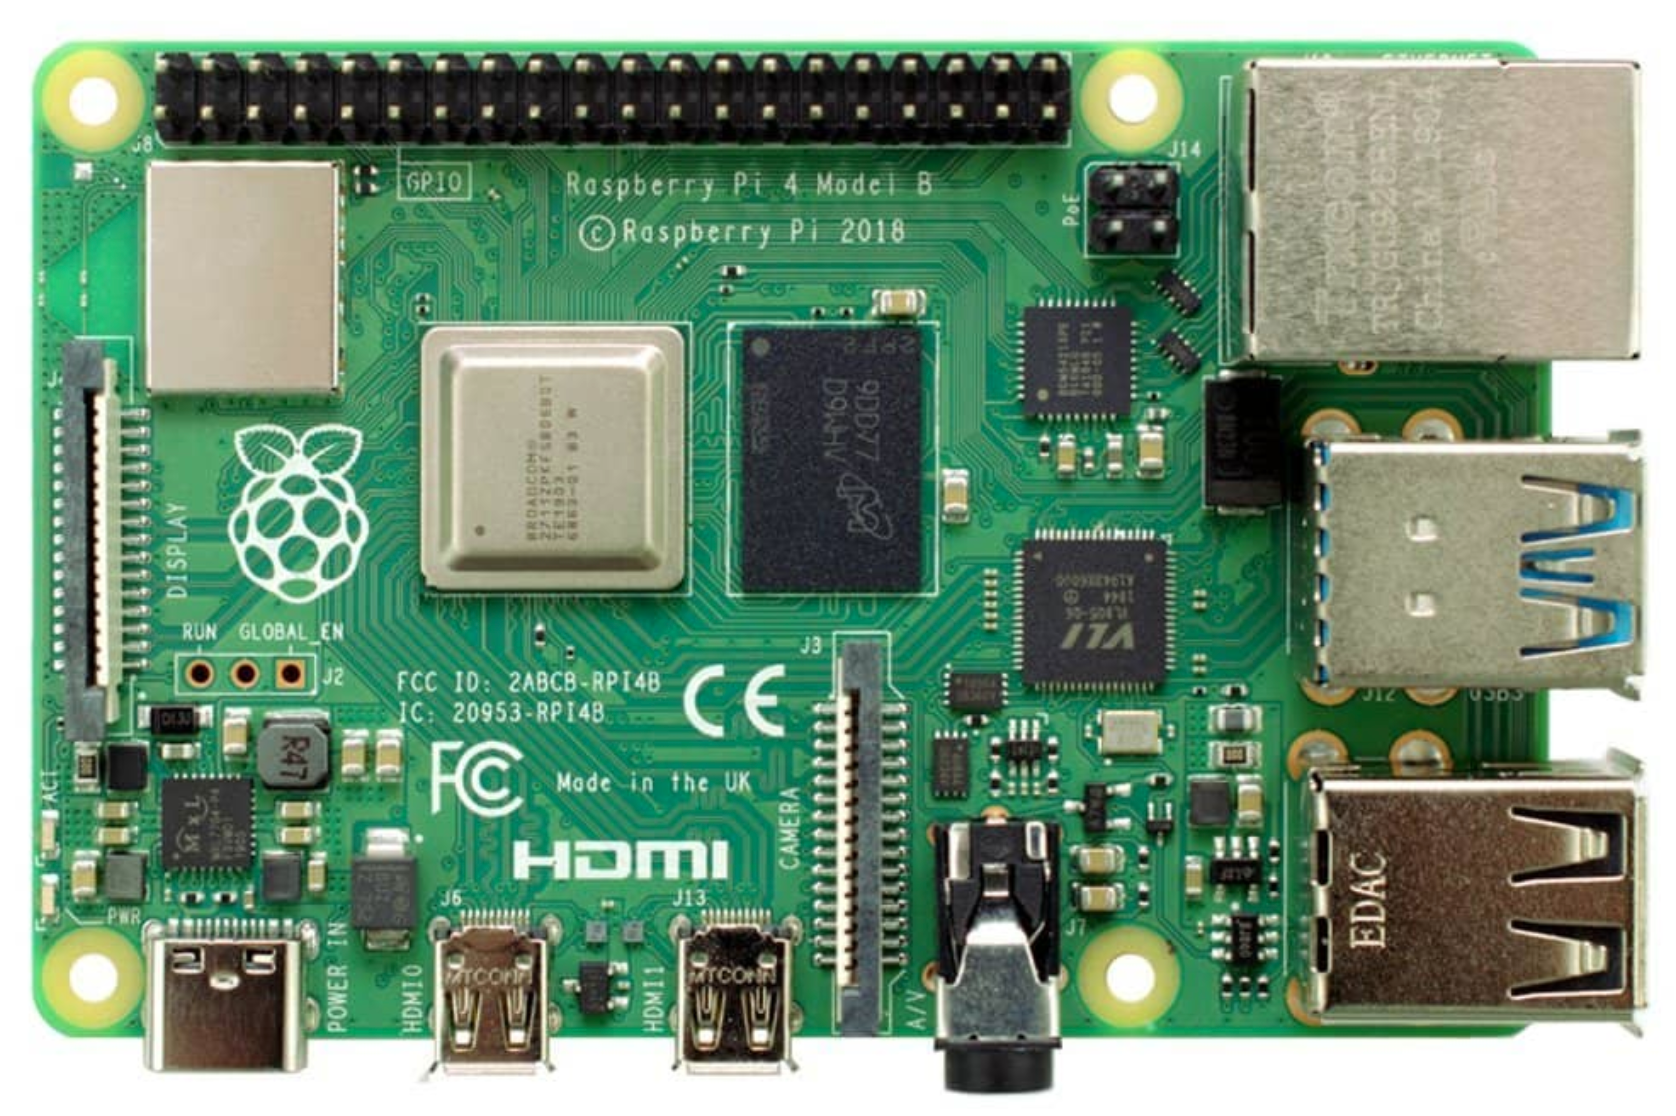
\includegraphics[width=.50\linewidth]{imagenes/raspberry_pi_2.png}
    \caption{Raspberry Pi 4 \cite{what_is_raspberry}.}
    \label{fig:raspberry}
\end{figure}

\subsubsection{Hologram Nova}
Modem celular diseñado para proveer de conectividad a internet (2G/3G/LTE-Cat-M1) a computadoras de una sola placa que utilicen alguna distribución de Linux como sistema operativo. Es ideal para aplicaciones de internet de las cosas que serán implementados en ubicaciones remotas. Al contratar el servicio se recibe por correo una tarjeta SIM con señal global. Esta se inserta en el USB que se conecta a la computadora para habilitar la conexión a internet. En la Figura \ref{fig:hologram_nova} se puede observar el dispositivo \cite{hologram_nova}.

\begin{figure}[!ht]
    \centering
    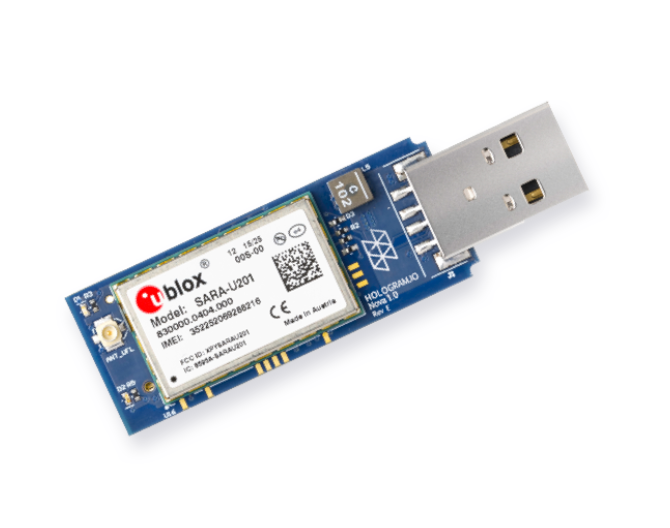
\includegraphics[width=.50\linewidth]{imagenes/hologram_nova_usb.png}
    \caption{Hologram Nova: modem celular \cite{hologram_nova}.}
    \label{fig:hologram_nova}
\end{figure}

\subsubsection{FastAPI}
\textit{Framework} minimalista para desarrollo de APIs REST en Python. Es uno de los \textit{frameworks} más rápidos disponibles para Python. Otra ventaja es que permite crear documentación compatible con el estándar OpenAPI automáticamente \cite{fastapi}.

\subsubsection{NGINX}
Servidor HTTP y de \textit{proxy} inverso utilizado mayormente por su capacidad de mantener en caché peticiones comúnes y balancear carga. Además, es capaz de funcionar como un servidor \textit{proxy} para servidores de correo (IMAP, POP, SMTP). Debido a su arquitectura escalable y su capacidad de actuar como un \textit{proxy} inverso, este servidor es utilizado comúnmente como un frente para otros servidores que no son tan eficientes. En estos escenarios es donde su capacidad de balancear carga al poder enviar peticiones a distintos servidores, dependiendo de la carga que tenga cada uno en el momento, lo diferencia de los demás servidores HTTP \cite{nginx}.

\subsubsection{PM2}
Administrador de procesos que ayuda a mantener servidores de aplicaciones en línea. Se desarrolló inicialmente para administrar servidores de Node.js, sin embargo, es capaz de administrar aplicaciones o procesos codificados en cualquier lenguaje \cite{pm2_landing}.

\subsubsection{MongoDB}
Motor de base de datos de código abierto no relacional que almacena los datos en objetos en notación de Javascript (JSON por sus siglas en inglés) llamados documentos. Los campos de los documentos pueden variar de documento a documento. Esta flexibilidad que ofrece contribuye a un desarrollo más rápido al no tenerse que preocupar de la integridad referencial. Tiene una licencia que permite su uso en aplicaciones personales y comerciales, siempre y cuando no se ofrezca la base de datos como un servicio \cite{what_is_mongo}.

\subsubsection{JSON Web Token}
Formato para comunicar afirmaciones entre dos partes de una manera segura para enviar en URLs. Las afirmaciones que contenga el \textit{token} están representadas como pares de llave/valor dentro de un JSON. Este puede ser firmado digitalmente por quien lo genere, protegiendo las afirmaciones originales de ser alteradas por algún actor externo \cite{jwt}.

\subsubsection{Vue.js}
\textit{Framework} reactivo de código abierto para crear interfaces de usuario en la web. Su arquitectura está diseñada para poder utilizarlo incrementalmente, su uso puede ir desde hacer pequeñas partes de la interfaz reactivas hasta desarrollar complejas aplicaciones de una sola página \cite{vuejs}. 


% TODO: El marco teorico es mas para 


% 4. Aplicaciones web
%     4.2 Bases de datos
%     4.3 APIs

